\RequirePackage[l2tabu, orthodox]{nag}
\documentclass[a4paper]{article}
\usepackage[utf8]{inputenc}
\usepackage[T1]{fontenc}
\usepackage{lmodern}
\usepackage[pdftex, hidelinks,
            pdftitle={Flödesanimering i Realtid med 3-D Curlbrus},
            pdfauthor={Martin Estgren and and Rasmus Hedin and Alfred Rundquist and Erik S. V. Jansson},
            pdfsubject={Computer Graphics -- Animation -- Physical Simulation / Procedural Animation},
            pdfkeywords={curl-noise,animation,fluid simulation,navier-stokes,gpu,real-time}]{hyperref}

\usepackage{bm}
\usepackage{caption}
\usepackage{listings}
\usepackage{mathtools}
\usepackage[margin=1.0in]{geometry}
\usepackage[parfill]{parskip}
\usepackage[swedish]{babel}
\usepackage{algorithmic}
\usepackage{graphicx}
\usepackage{courier}
\usepackage{hyperref}
\usepackage{amsmath}
\usepackage{amssymb}
\usepackage{algorithm}
\usepackage[capitalize, noabbrev]{cleveref}
\usepackage[activate={true, nocompatibility}, final,
            tracking=true, kerning=true, spacing=true,
            factor=1100, stretch=10, shrink=10]{microtype}

\DeclareCaptionFormat{modifiedlst}{\rule{\textwidth}{0.85pt}\\[-2.9pt]#1#2#3}
\captionsetup[lstlisting]{format =  modifiedlst,
labelfont=bf,singlelinecheck=off,labelsep=space}
\lstset{basicstyle=\footnotesize\ttfamily,
        breakatwhitespace = false,
        breaklines = true,
        keepspaces = true,
        language = C++,
        showspaces = false,
        showstringspaces = false,
        frame = tb,
        numbers = left,
        numbersep = 5pt,
        xleftmargin = 16pt,
        framexleftmargin = 16pt,
        belowskip = \bigskipamount,
        aboveskip = \bigskipamount,
        escapeinside={<@}{@>}}

\date{\vspace{-1.8ex}} % Buys us some space.
\title{\vspace{-2.2cm}\textbf{Flödesanimering i Realtid med 3-D Curlbrus}\\
       \Large{\textit{--- en kort teknisk saga angående dess fasor och dess under ---}}}
\author{{\textbf{Martin Estgren}}\;\;\;\;\;\; {\href{mailto:mares480@student.liu.se}{\texttt{<mares480@student.liu.se>}}}\\
        {\textbf{Rasmus Hedin}}\;\;\;\;\;\;\;\; {\href{mailto:rashe877@student.liu.se}{\texttt{<rashe877@student.liu.se>}}}\\
        {\textbf{Alfred Rundquist}}\;\;\; {\href{mailto:alfru536@student.liu.se}{\texttt{<alfru536@student.liu.se>}}}\\
        {\textbf{Erik S. V. Jansson}}\; {\href{mailto:erija578@student.liu.se}{\texttt{<erija578@student.liu.se>}}}}

\begin{document}
    \maketitle

    \section{Motivering samt problem}

    Ett viktigt område inom datorgrafik och visualisering är förmågan att kunna simulera verklighetstrogna flödessystem i realtid. I detta projekt har vi implementerat grundläggande flödesystem för ett partikelsystem i 3D via en metod kallad \textit{Curl-nosie} först presenterat av Robert Bridson et al.\cite{bridson2007curl}.

    \textit{Curl-noise} är en metod att framställa verklighetstroget partikelflöde genom att procentuellt animera turbulenta flöden genom med hjälp utav procentuellt brus som man applicerar några relativt billiga operationer på, istället för att beräkna flödet det genom t.ex. \textit{Navier-Stokes ekvationer}. 

        \subsection{Mål och avgränsningar}

        \subsection{Arbetsprocess och verktyg}

    \section{Teori och implementering}

        \subsection{Systemöversikt}

        \subsection{Partikelsystemet}

    Flödets riktning beräknas för varje partikels position genom följande system. I original papperet presenteras både beräkningarna för två och tre dimensioner men eftersom vi valt att enbart implementera den sistnämnda fokuserar vi på den. Vi kommer ej heller följa originalpapperets beräkningar exakt utan justerar så det passar vårat system bättre.

    \textbf{Brusriktningen}
    \begin{equation}
   N(\vec{x}) =  
        \begin{pmatrix}
        n((\vec{x} + \vec{\epsilon}_x)/L)
        \\
        n((\vec{x} + \vec{\epsilon}_y)/L)
        \\ 
        n((\vec{x} + \vec{\epsilon}_z)/L)
        \end{pmatrix} * \gamma M_nL
    \end{equation}
    Där $\vec{\epsilon}$ representerar en förskjutning så att inte alla komponenter får exakt samma värde, i detta fall $\vec{\epsilon} = \begin{bmatrix}
8 & 0 & 0\\ 
0 & 8 & 0\\ 
0 & 0 & 8
\end{bmatrix}$. $n(\vec{x})$ är brusfunktionen som samplas för att producera turbulens i fältet. Vi valde att använda \textit{Simplex noise}\footnote{\url{http://webstaff.itn.liu.se/~stegu/simplexnoise/simplexnoise.pdf}}. $\gamma$ representerar förhållande mellan brus och bakgrundsfällt där $0$ är inget brus och därmed ingen turbulens medan $1$ är fullt brus utan något bakgrundsfällt. $M_n$ är styrkan på bruset (Fällriktningen är normerad så vi skalar upp det till vad vi vill ha). $L$ är längdskalan på bruset vilket i vårat fall är relativt stor (20-100) då vi vill ha långa övergångar i bruset.

\textbf{Bargrundskikningen}
\begin{equation}
    F(\vec{x}) = (1.0-\gamma) * D(\vec{x}) * M_f
\end{equation}
$D(\vec{x})$ representerar fällriktningen i den angivna punkten. Fällriktningen är beräknad enligt följande formel
\begin{equation}
   D(\vec{x}) = \vec{x} \times \vec{p}
\end{equation}
Där $\vec{p}$ är fällriktningen vi är ute efter. Eftersom $\bigtriangledown \times$ roterar alla vektorer med $\pi/2$ behöver vi först rotera fällriktning själva så att efter $\bigtriangledown \times$ riktningen blir $\vec{p}$.

Brusriktningen adderas med bargrundskikningen för att sedan justeras så den beaktar solida sfärer utplacerade i vektorfältet $\vec{\psi} = N(\vec{x} + F(\vec{x})$.

\textbf{Alpha}
För att få alla partiklar att respektera de sfärer vi placerat i fältet använder vi en rampfunktion.
\begin{equation}
ramp(r) = \left\{\begin{matrix}
1  && r > 1
\\
10r^3 + 6r^4 && 0 \le r \le 1
\\ 
0  && r < 0
\end{matrix}\right.
\end{equation}
där $r$ är skillnaden mellan distansen $\vec{x}$ och den närmsta sfären delat på marginalen runt sfären. 

För att få partiklarna att gå runt sfärerna använder vi nu resultatet från ramp funktionen som $\alpha = | ramp(d(\vec{x})/d_0) |$ där $d_0$  är en arbiträr skalfaktor. Slutligen beräknar vi hur fältet runt sfären ska se ut genom 
\begin{equation}
\vec{\psi}_c(\vec{x}) = \alpha * \vec{\psi}(\vec{x}) + (1.0 - \alpha) * \vec{x} * \vec{\psi}(\vec{x}) \cdot \vec{x}
\end{equation}
vilket producerar en övergång från fällriktningen till en riktning enbart är normalen från fältet mot sfären.

\textbf{Curl}
Vi får fram $\bigtriangledown \vec{\psi}$ genom \textit{finite difference}
\begin{equation}
\vec{vx} = \vec{\psi}_c(\vec{x} + \vec{\epsilon}_x  ) - \vec{\psi}_c(\vec{x} - \vec{\epsilon}_x  )
\end{equation}
\begin{equation}
\vec{vy} = \vec{\psi}_c(\vec{x} + \vec{\epsilon}_y  ) - \vec{\psi}_c(\vec{x} - \vec{\epsilon}_y  )
\end{equation}
\begin{equation}
\vec{vz} = \vec{\psi}_c(\vec{x} + \vec{\epsilon}_z  ) - \vec{\psi}_c(\vec{x} - \vec{\epsilon}_z  )
\end{equation}
där $\vec{\epsilon} = \begin{bmatrix}
0.0001 & 0 & 0\\ 
0 & 0.0001 & 0\\ 
0 & 0 & 0.0001
\end{bmatrix}$ och varje resultatvektor $\vec{vx},\vec{vy},\vec{vz}$ är de partiella derivatorna i punkten $\vec{x}$.

Slutligen beräknas den slutgiltiga fältriktningen genom att applicera curl operatorn på vår framtagna gradient genom
\begin{equation}
\bigtriangledown \times =\frac{\begin{pmatrix}
vy_z - vz_y
\\ 
vz_z - vx_y
\\ 
vx_z - vy_y
\end{pmatrix}}{0.0002}
\end{equation}
och normeras så att vi själva kan bestämma vad hastigheten för partiklarna ska vara.

        \subsection{Partikelrenderaren}

        \subsection{Övriga funktioner}

    \section{Resultat och diskussion}

\begin{figure}[H]
\center
\begin{minipage}[]{0.19\textwidth}

\includegraphics[width=\textwidth]{share/Noise.png}
\end{minipage}
\begin{minipage}[]{0.19\textwidth}

\includegraphics[width=\textwidth]{share/Background.png}
\end{minipage}
\begin{minipage}[]{0.19\textwidth}

\includegraphics[width=\textwidth]{share/Alpha.png}
\end{minipage}
\begin{minipage}[]{0.19\textwidth}

\includegraphics[width=\textwidth]{share/Potential.png}
\end{minipage}
\begin{minipage}[]{0.19\textwidth}
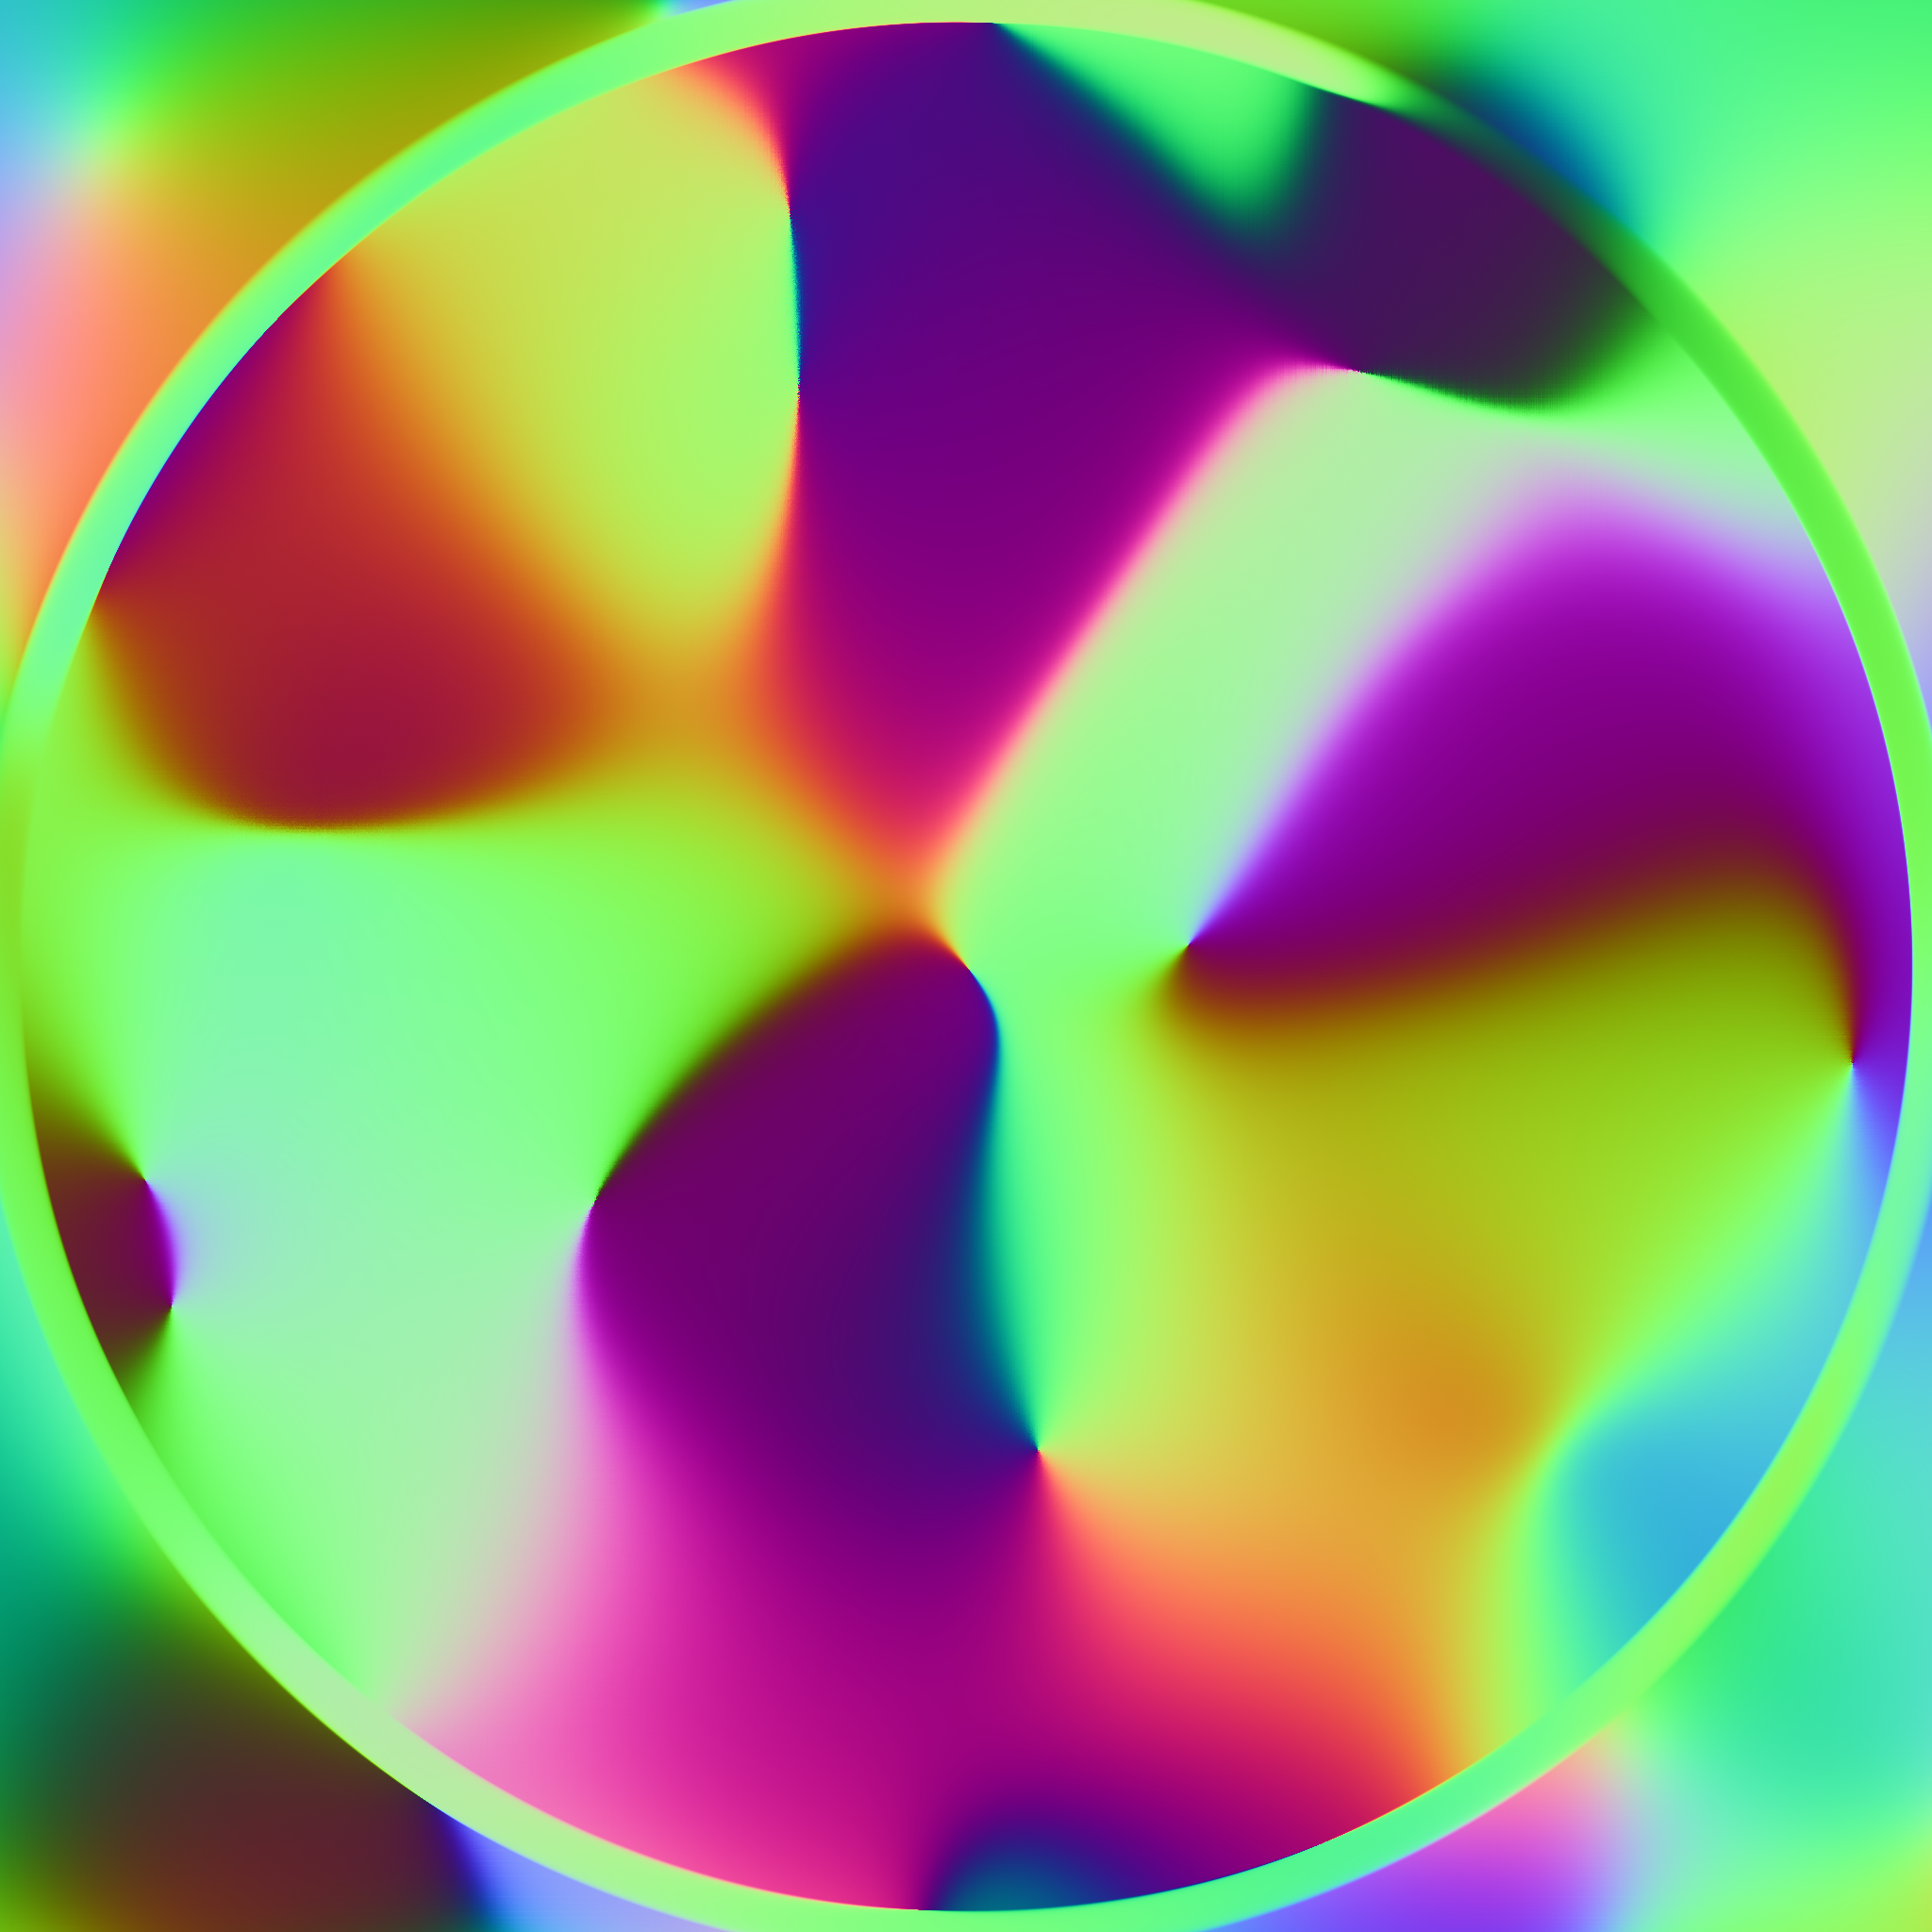
\includegraphics[width=\textwidth]{share/Curl.png}
\end{minipage}
\end{figure}

        \subsection{Problem och Lösningar}

        \subsection{Framtida förbättringar}

        \subsection{Projektreflektioner}

    \nocite{*} % Include all.
    \bibliographystyle{abbrv}
    \bibliography{cnpf}

\end{document}
